%!TEX encoding = UTF-8 Unicode
%!TEX program = xelatex

\documentclass[bachelor,fontset=windowsold]{ustcthesis}
% bachelor|master|doctor
\usepackage{ustcextra}
\graphicspath{{figures/}}
\bibliographystyle{ustcauthoryear}
% \bibliographystyle{ustcnumerical}

\title{中国科学技术大学\\基于搜索引擎的短文本视觉表达的研究}
\author{黄红艳}
\major{计算机科学与技术}
\advisor{孙广中\ 副教授}
\submitdate{二〇一七年五月}
%\secrettext{机密\quad 小于等于20年}   % 内部|秘密|机密,注释本行则不保密
\depart{十一系}

\entitle{Visual Expression for Short Text Base on Search Engine}
\enauthor{Hongyan Huang}
\enmajor{Computer Science and Technology}
\enadvisor{A.P. Guangzhong Sun}
\ensubmitdate{May, 2017}
%\ensecrettext{Confidential\quad Less than or equal to 20 years}  % Internal|Secret|Confidential

%ADD——hhy
%\newcommand{\tabincell}[2]{\begin{tabular}{@{}#1@{}}#2\end{tabular}}
\usepackage{multirow,array}

\begin{document}

\maketitle

%
% 本科论文:
%   frontmatter: 致谢、目录、中文摘要、英文摘要
%   mainmatter: 正文章节、参考文献
%   appendix: 附录
%
% 硕博论文:
%   frontmatter: 中文摘要、英文摘要、目录、符号说明
%   mainmatter: 正文、参考文献
%   appendix: 附录
%   backmatter: 致谢、发表论文
%

\frontmatter
\begin{acknowledgements}

在研究学习期间,我有幸得到了三位老师的教导,
他们是:我的导师,中国科大孙广中研究员,微软亚洲研究院谢幸老师和宋睿华老师。
三位深厚的学术功底,严谨的工作态度和敏锐的科学洞察力使我受益良多。
衷心感谢他们多年来给予我的悉心教导和热情帮助。

感谢宋睿华老师在实验方面的指导和帮助。
科大的李顶龙同学和陈仲夏同学参与了部分试验工作,在此深表谢意。

\end{acknowledgements}

\tableofcontents
\begin{abstract}
短文本囿于字数极少,这使得人在理解时会联系到各种感官经验,这其中就包括视觉。比如“猴子爬树”,我们在理解时会联想到树木的图像。本课题旨在利用搜索引擎,对一段短文本能否使用图像表达进行探究。本课题试图解决以下几个问题:第一,定义短文本的视觉表达;第二,通过调查问卷,人工标记具体短文本是否能视觉表达;第三,通过监督学习的方法,自动识别能视觉表达的短文本。
	

\keywords{近似搜索\zhspace{} 图片搜索\zhspace{} 可视化\zhspace{}询问分类}
\end{abstract}

\begin{enabstract}
The short text is limited by the few words, which makes it possible for people to understand the sensory experience, which includes vision. For example, "monkeys climb trees", we will understand the tree when the image. This topic aims to use the search engine, a short text can use the image expression to explore. This question attempts to solve the following questions: First, the definition of short text of the visual expression; Second, through the questionnaire, manually marked the specific short text can be visual expression; Third, through the supervision of learning methods, automatic identification of visual expression The short text.


\enkeywords{Similarity Search, Image Retrieval, Visualization, query classification}
\end{enabstract}


\listoffigures
\listoftables
\listofalgorithms  % 算法索引,如不需要,可直接注释掉本行
% \begin{notation}

\centering
\begin{tabular}{rl}
$\ln x$ & natural logarithm $\log_ex$ \\
$\log x$ & common logarithm $\log_{10}x$ \\
$x\ \mathrm{mod}\ y$ & remainder \\
\end{tabular}

\end{notation}


\mainmatter
\chapter{简介}
\section{模板简介}
测试脚注\footnote{分别编号}。

\subsection{模板介绍1}

\subsubsection{模板测试}

\subsection{模板介绍2}

\section{系统要求}

\section{问题反馈}
测试脚注\footnote{脚注2}

\chapter{短文本对话Short Text Conversation}

\begin{table}[htbp]
\centering
\caption{新浪微博一个典型帖子Post和它的评论Comment} \label{tab:example_STC}
\begin{tabular}{|c|p{10cm}|}
    \hline
    \textbf{Post} & 创新工场三年庆,在我们的「智慧树」会议室。\par Today is the 3-year anniversary of Innovation Works. We are in the meeting room named Tree of Wisdom.  \\
    \hline
    \textbf{Comment 1} & 时间过得真快,创新工场都3年了!周年庆快乐!\par How time flies; Innovative Works is three years old! Happy Anniversary!\\
    \hline
	\textbf{Comment 2} & 小小智慧树,快乐做游戏,耶!\par Little Wisdom Tree, happy games, yeah! \\
	\hline
	\textbf{Comment 3} & 会议室挺气派,顶一个!\par The meeting room is quite impressive, the best one! \\
	\hline
\end{tabular}
%\note{这里是表的注释}
\end{table}
人与电脑之间的自然语言交流是最具挑战性的AI问题之一,涉及语义理解,推理和常识知识的运用。尽管过去几十年来对人机交互研究工作进行了大量的努力,但令人遗憾的是,这个问题的进展非常有限。其中一个主要原因是缺乏大量的真实对话数据。

在短文本对话任务中,我们只考虑一个简化版本的问题:由两个短文组成的一轮对话,前者是用户的初始帖子,后者是计算机给出的评论。我们把它称为短文本对话(STC)。由于在Twitter和微博等社交媒体上提供了大量短文本对话数据,我们预计在使用大数据的问题研究中可以取得重大进展,就像在机器翻译,社区问答等领域一样。随着社交媒体的出现和移动设备的广泛传播,通过短消息的对话已成为重要的沟通方式。许多现实中应用可以从短文本对话的研究中受益,例如手机上的自动消息回复,Siri等语音助手以及用于智能家居设备上各种聊天机器人。

在NTCIR-12上短文本对话的作为试点任务提出,让有兴趣的自然语言对话的研究人员聚在一起。在NTCIR-12,短文本对话(STC)被认为是一个信息检索(IR)问题,通过在日语子任务中保持一个大量的Twitter中的子博客Twitter和Twitter Twitter的留言对,然后找到一个聪明的方法来重用这些现有的评论来回应新的帖子。在中文子任务中,语料库来自于微博。

在今年我参加的NTCIR-13中,除了基于检索的方法之外,主办方还考虑了基于生成的方法来生成“新”评论。基于生成的方法已经成为一个热点研究课题,近年来受到最多的关注,而基于检索的方法是否完全被替代或者与基于生成的短文本对话(STC)任务的方法组合在一起仍然是一个开放的问题。NTCIR-13的短文本对话任务提供了一个透明的平台,通过进行综合评估来比较基于检索和基于新生成方法。此外,主办方鼓励参与者探索一些有效的方式来结合两种方法来获得更智能的聊天机器人。

短文本对话(STC)的一个简单方法,也许是大部分人第一种想要尝试的方法,就是将其作为信息检索(IR)问题:维护一个大型的短文对话数据库,并开发主要基于信息检索(IR)技术的会话系统。给定一个初始帖子(Post)A,系统搜索语料库并返回最合适的评论(Cmt)。存储库中的评论(Cmt)最初是针对Post A以外的一些帖子发布的,但我们假设语料库足够大,包含了所有可能存在的帖子(Post),因此我们假设可以将其重新用于对A的合理评论(Cmt)。也就是说,我们处理更简单的基于检索的短文本对话(STC),而不是追求基于生成的短文本对话(STC),即从用户的初始帖子(Post)生成适当的评论(Cmt)。利用先进的信息检索(IR)技术和大数据,即使是基于检索的短文本对话(STC)系统也可能在每一轮会话中最终都会像人类一样表现出来。

\subsection{任务描述}
在本文的研究中,我们将短文本对话定义为一个信息检索问题,即基于检索的短文本对话。存储库我们也称为语料库,是有来自于微博的帖子-评论(Post-Cmt)对。在表\ref{tab:example_STC}中显示了一个微博帖子和三个对应它的评论。每个参赛队伍都会收到主办方事先准备好的语料库。值得注意的是,不仅一个帖子会对应多个评论,在对评论进行去重复处理编号后,会有不少评论对应了多个帖子。

%\item 
在\textbf{训练}期间,主办方会发布训练数据,他们是被人工标记评级过的帖子-评论对。关于人工标记评级,将在下一节阐述。我们要使用之间收到的语料库和这些被标记过的帖子-评论对作为训练数据,构造一个会话系统。
 
%\item 
在\textbf{测试}期间,每个参赛队伍对收到一个测试集,由一下微博帖子组成,每个帖子都被保证不在语料库中。我们需要为每个测试帖子提供十个结果(评论)的排名列表,而且这些评论必须来自于语料库。

%\item 
在\textbf{评估}期间,所有参赛团队提交的结果都会被匿名集合到一起人工标记。评估会使用信息检索分级相关的测量方法。

在表\ref{tab:statistics_STC}显示了中文子任务中数据集的统计结果。在语料库中有差不多20万条微博帖子,每个帖子平均有30条评论,但是大概有100万帖子-评论对中的评论重复。主办方标记了225个帖子的作为训练数据,每个帖子平均大约有30个候选评论。有100个帖子作为测试数据,这些用于测试的帖子保证不再语料库中,参赛者需要搜索自己的会话系统,为每个测试帖子寻找10个评论和其排名作为结果。微博上原始网页的文本是中文的,为了帮助非华人参赛者,主办方提供了英文版本,所有的英文翻译都来自于机器翻译。华人参赛者也能收到英文版本作为参考。


\begin{table}[htbp]
\centering
\caption{STC中文子任务数据集统计} \label{tab:statistics_STC}
\begin{tabular}{|p{4cm}|l|r|}
    \hline
    \multirow{3}{4cm}{语料库 \linebreak Retrival Repository} & \#Posts & 196,495 \\ 
	\cline{2-3}
	& \#Comments & 4,637,926 \\ 
	\cline{2-3}
	& \#original pairs & 5,648,128 \\ 
	\hline
	\multirow{3}{4cm}{标记数据 \linebreak Labeled Data} & \#Posts & 225 \\ 
	\cline{2-3}
	& \#comments & 6,017 \\ 
	\cline{2-3}
	& \#labeled pairs & 6,017 \\ 
	\hline
	测试数据 Test Data & \#query posts & 100 \\
	\hline
\end{tabular}
%\note{这里是表的注释}
\end{table}
	
	
%\subsection{相关评估}

\subsection{研究想法}
因此,我们想研究的关键问题是:给定一个新的帖子(Post),如何搜索语料库来返回适当的(即类似人的)评论?陈仲夏师兄,在NTCIR-12上给出了他的想法:假设语料库

在我的论文研究中,主要针对信息检索的方法的前期工作,研究短文本的视觉表达提供了一种新的检索语料库的
%短文本对话是指根据一段短文字,计算机模仿人类给出连贯的有意义的回复。过去文本都是从语料库中找寻合适的回答,近些年随着机器学习的发展,循环神经网络RNN和长短周期神经网络LSTM的出现文字转向量Word2Vec技术的成熟,文本生成技术是的生成文本回复短对话有种有短文本对话是当下热门的研究方向,以微软小冰、苹果Safari为代表,各家互联网公司都在积极研发对话机器人。现在得到对话问答





\chapter{视觉表达}
短文本对话希望根据一段短文字,计算机模仿人类给出连贯的有意义的回复。人类在对一段文字进行回复的时候会经历:理解问题——大脑思考——给出回答,这样的一个过程。但是怎么判断别人(或者计算机)是否真正理解了你的意思?这个问题似乎很难回答。在目前自然语言理解领域上,对其有两个定义,一个是基于行为的,一个是基于表示的。对于前者,如果你说“给我拿一杯茶来”,别人(机器人)真的按你说的做了(行为),就认为他了解了你的意思;而对于后者,如果你说“猴子爬树”,别人把它联系到了大脑中猴子爬树的概念(表示),就认为他理解了你的意思。

%(如图\ref{fig:robot_tea})

十几年前,脑科学研究中有一个有趣的发现。当把电极插到猴子的大脑前运动皮质(pre-motor cortex)时,有一个脑细胞会在猴子自己吃香蕉和看别人吃香蕉时,同样处于兴奋状态,也就是说对猴子来说这个脑细胞对应着“吃香蕉”的概念。(猴子和人的运动都是由小脑控制, 但大脑的前运动皮质也与运动有关。)后来对人脑做类似的实验,但使用功能磁共振。让人实际做和想象做各种动作,比如跑步和想象跑步,爬树和想象爬树。结果发现,对同一动作,实际做和想象做大脑的前运动皮质中发生反应的部位完全一致。现在一个得到广泛支持的理论认为,对于同一个概念,大脑用固定的脑细胞去记忆,人理解语言的过程,就是激活相关概念的脑细胞,并关联这些概念的过程表示同一个概念的脑细胞,可以通过不同的方式被激活。例如,有一个细胞表示人在喝水,当你看到人在喝水的时候,或者当你从书中读到人在喝水的时候,这个脑细胞同样会被激活。这也能解释为什么我们在读小说的时候常常有身临其境的感觉。

每个人把自己经历的事件进行编码,存储记忆在脑细胞中,在与外界的交互中这些脑细胞被激活,相关的记忆被唤醒。所以,不同人对同样的语言会有不同的理解,因为他们的经历不同。但也有许多共性,因为大家在交流过程中,相互激活对方脑中的表示相同内容的细胞。发明比喻的时候,大脑中表示两个不同概念的部位都开始兴奋,相关的脑细胞之间产生新的连接,概念之间产生关联,这个过程被称为神经结合(neural binding),是现在脑科学研究的重要课题\footnote{Lakoff G. What Studying the Brain Tells Us About Arts Education, 2013.}。

语言的理解实际上是一个非常复杂的过程,动用了各种各样的感官,动用了大脑中所有的相关知识。我们的研究想让计算机读到一个短文本的时候能模拟人读到它的时候大脑产生的概念。这个过程就像是一个刚刚渡过婴儿期开始定义这个世界的孩子,她一开始一定没有“树”概念,她是在见过许多现实中的树,照片中的树,图画中的树之后才有了“树”的概念。也就是说,这样的概念其实是来自于这个孩子的视觉感受,当她在产生“树”的概念时是这些视觉图像的浓缩。正如“树”在脑海中会浮现出一个“树”的图片,我们在看到一段短文本对其产生概念,会在脑海中产生视觉图像,当然这样的视觉图像并不是在所有的短文本上就会产生,比如“昧着良心”。因此我们认为,\textbf{当我们读到一段短文字,对其产生的概念是否能用图像表示定义为短文本的视觉表达}。
\begin{figure}[ht]
\centering
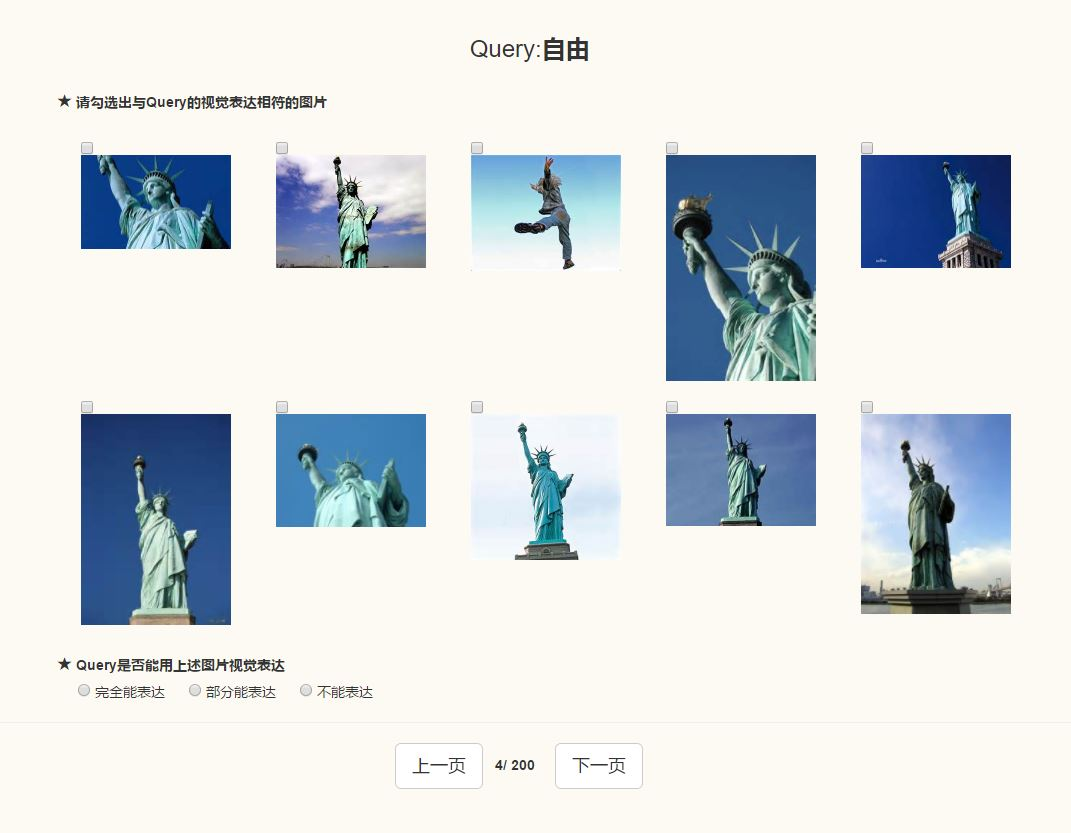
\includegraphics[width=14cm]{quest_vision}
\caption{单词视觉表达问卷调查} \label{fig:quest_vision}
\end{figure}
对于对话系统来说,它在看到一段短文本时,产生概念是什么?对于计算机来说。我们可以通过图片搜索引擎轻易地将短文本转化成图像集合。但是怎么判断这些图像集合能否等价于其视觉表达呢?我们将每个进行图片搜索的短文本称为一个查询用Query表示,将图片搜索得到的结果进行了人工标注如图\ref{fig:quest_vision}。标注员能够在一个页面里看到Query(查询)的短文本,和Query(查询)通过图片搜索得到的图片集合。标注员需要回答Query(查询)是否能用上述图片视觉表达以及勾选出符合标注员对短文本产生概念的视觉表达的图像。经过反复的人工标记,我们得到了以下准则:
\begin{itemize}
	\item     Query(查询)经过图片搜索得到的图片能够与其查询的短文本在人脑海中联系的的视觉表达相关,视为图片能作为Query(查询)的视觉表达。
	\item  当Query(查询)经过图片搜索得到的图片能作为Query(查询)的视觉表达的数量足够多时,视为与Query的意思能用图片视觉表达,数量不够的时候视为Query的意思能用上述图片部分视觉表达
	\item   当搜索得到的图片集有多个相同的语义时,当短文本的语义存在多个时,以及当符合Query(查询)视觉表达的图片数量不够多时,都视为Query能用搜索得到的图片集部分视觉表达
	\item    当搜索得到的图片集数量不足,或者图片杂乱无章时,视为Query(查询)不能用图片视觉表达。
\end{itemize}

在反复标记的过程中我们发现很多有趣的东西。除了我们很容易联想到的一些生活中的物品比如笔,树有视觉表达,在图\ref{fig:quest_vision}中,我们定义的一些在现实中没有的虚无的东西,也找了一致表达。在这个例子中图片搜索引擎返回给我们了很多自由女神像的图片,这跟我们人类的常识相符,我们使用自由女神像来代表自由,这是我们想要的在文字之外的关联。在另一个层面说,我们想要通过搜索引擎来寻找短文本一致的视觉表达。我们认为如果一个Query(查询)返回的图片越多一致的图片,这个图片是其人在脑海中的视觉表达概率越高。

另一个有意思的例子是Query:“玉米”的消费力,这样的一个Query(查询)在图片搜索后得到的结果是李宇春演唱会的图片。“玉米”除了是我们知道的食物之外,还是李宇春粉丝团的名字。在经过图片搜索引擎视觉表达后,像是经过了一轮人的思考和联系之后得到的视觉表达。同样的例子还出现在,在对帖子进行视觉表达后聚类中,关于食物话题的帖子的视觉表达会聚类在一起。我们认为经过图像表达可以比文字更能表示贴近我们脑海中的形象。

为了区别于Post(帖子),我们特意使用了Query(查询)来表示用于图片搜索的短文本。在本文的研究中,我们为了使Post(帖子)能够更好的进行图像表达,后续的相关章节会讨论关于帖子怎么变成Query(查询)。

在我们想设计的对话系统想要模拟人在理解短文本过程中是否利用到了我们的视觉感官系统。我们通过将短文本(帖子)变成一些相关的Query(查询),将Query(查询)得到图片集定义为计算机能够理解的短文本的视觉表达。

\subsection{图片搜索引擎}
由于搜索引擎已经花费了大量精力来完善他们官方使用的图像检索服务,我们可以很轻易收集标签图像。我们可以通过搜索图像标题、文件名和周围文本等方式来检索图像。现在各大图片搜索引擎都提供了搜索图片的API,要实现自动检索图像,我们可以将一个单词或短语(本文我们统一称为Query查询)作为HTTP查询提供给搜索引擎,并直接下载所返回的均匀缩略图,而不是直接下载原图像。一个是因为源网站图像要返回源网站下载,所以不如缩略图稳定;二是最后可能涉及的查询Query数量很多,考虑到存储空间;三是为图像大小相对均匀,这样在提取特征和问卷调查时候需要考虑图片差别。

各大图片搜索引擎提供的自动检索的接口都设置了流量限制,而我们的研究和对话系统数量较大,我们的研究经费难以承担。在宋睿华老师的帮助下,我们的难题得到了解决。因此本文的研究都使用Bing的图像搜索作为搜索引擎(https://www.bing.com/images)。我们的自动检索接口检索所得图片和人工检索结果一致。

\subsection{图片集数量}

我们希望通过图片搜索后的图片的集合来代表Query查询的图像表达。但是,显然我们不能将所有的图片缩略图都下载下来。一个是程序运行时间和存储限制,第二个是人工标记也不能顾上。我们当然希望能用最少的图片集数量来判断一个查询是否能够用视觉代表。

\begin{figure}[ht]
\centering
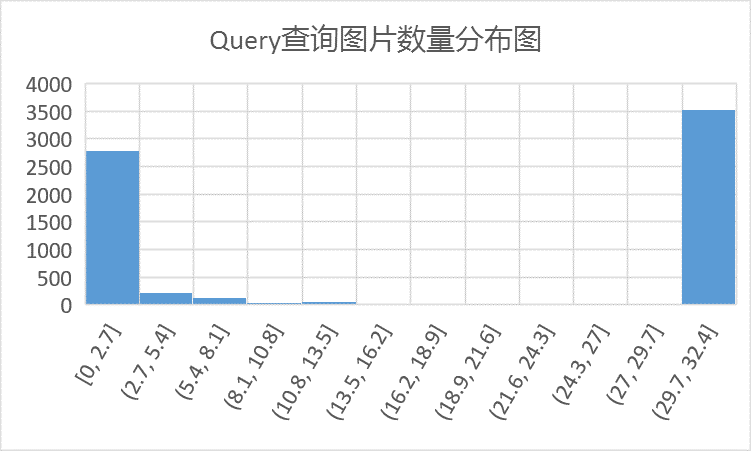
\includegraphics[width=10cm]{ImageNum_Test}
%\note{查询图像数量分布图}
%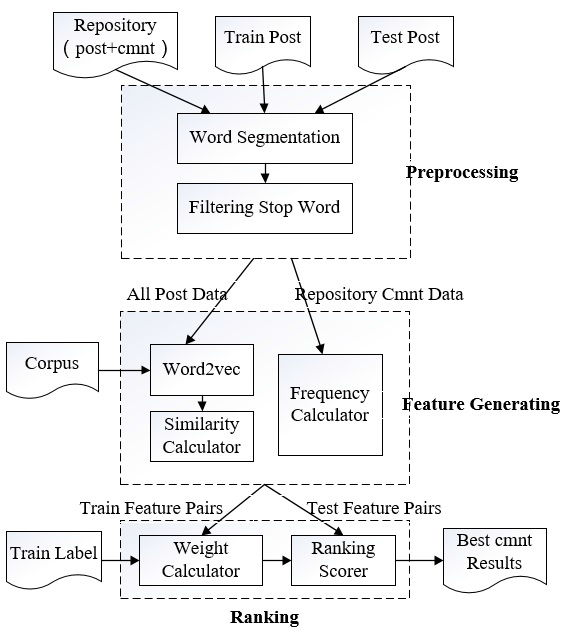
\includegraphics[width=10cm]{Chen_Architecture}
\caption{查询图像数量统计} \label{fig:ImageNum_Test}
\end{figure}

因此我们测试帖子进行分词后将帖子所有可能长度进行了分割。也是说,如果一个帖子有N个单词,我们可以将帖子分成N*(N-1)/2个Query(查询)。因此,现在的查询集合包含了所有可能长度。我们将图片搜索引擎的返回图片数量设置到30,记录每条Query查询的返回图片数量。100个测试帖子共分成了6,872个Query(查询),查询的最大词数是58,最小词数为1。返回图片数量如上图\ref{fig:ImageNum_Test}所示,图片数量集中在最小值0和最大值30,在图片数量在10附件可以涵盖大部分Query查询。为了尽可能少的下载图片数量,本文中搜索引擎中一个Query查询取回的图片最大数量为10。







\chapter{单词的视觉表达}




\chapter{图片}
本章展示图片相关用法。

\section{示例}
\begin{figure}[ht]
\centering

\includegraphics[width=10cm]{ustc_logo_fig}
\caption{测试图片} \label{fig:figure1}
\end{figure}

\section{带图注的图}
\begin{figure}[ht]
\centering

\includegraphics[width=10cm]{ustc_logo_fig}
\caption{带图注的图片}\label{fig:noted-figure}
\note{the solid lines represent the time histogram of the spontaneous activities of an old monkey cell(gray) and a young monkey cell (black). The bin-width is 1}
\end{figure}

\chapter{表格}

\section{A Simple Table}
\begin{table}[htbp]
\centering
\caption{这里是表的标题} \label{tab:simpletable}
\begin{tabular}{|c|c|}
    \hline
    a & b \\
    \hline
    c & d \\
    \hline
\end{tabular}
\note{这里是表的注释}
\end{table}

\section{长表格}
\begin{longtable}{ccc}
% 首页表头
\caption[长表格演示]{长表格演示} \label{tab:longtable} \\
\toprule[1.5pt]
名称  & 说明 & 备注\\
\midrule[1pt]
\endfirsthead
% 续页表头
\caption[]{长表格演示(续)} \\
\toprule[1.5pt]
名称  & 说明 & 备注 \\
\midrule[1pt]
\endhead
% 首页表尾
\hline
\multicolumn{3}{r}{\small 续下页}
\endfoot
% 续页表尾
\bottomrule[1.5pt]
\endlastfoot

AAAAAAAAAAAA   &   BBBBBBBBBBB   &   CCCCCCCCCCCCCC   \\
AAAAAAAAAAAA   &   BBBBBBBBBBB   &   CCCCCCCCCCCCCC   \\
AAAAAAAAAAAA   &   BBBBBBBBBBB   &   CCCCCCCCCCCCCC   \\
AAAAAAAAAAAA   &   BBBBBBBBBBB   &   CCCCCCCCCCCCCC   \\
AAAAAAAAAAAA   &   BBBBBBBBBBB   &   CCCCCCCCCCCCCC   \\
AAAAAAAAAAAA   &   BBBBBBBBBBB   &   CCCCCCCCCCCCCC   \\
AAAAAAAAAAAA   &   BBBBBBBBBBB   &   CCCCCCCCCCCCCC   \\
AAAAAAAAAAAA   &   BBBBBBBBBBB   &   CCCCCCCCCCCCCC   \\
AAAAAAAAAAAA   &   BBBBBBBBBBB   &   CCCCCCCCCCCCCC   \\
AAAAAAAAAAAA   &   BBBBBBBBBBB   &   CCCCCCCCCCCCCC   \\
AAAAAAAAAAAA   &   BBBBBBBBBBB   &   CCCCCCCCCCCCCC   \\
AAAAAAAAAAAA   &   BBBBBBBBBBB   &   CCCCCCCCCCCCCC   \\
AAAAAAAAAAAA   &   BBBBBBBBBBB   &   CCCCCCCCCCCCCC   \\
AAAAAAAAAAAA   &   BBBBBBBBBBB   &   CCCCCCCCCCCCCC   \\
AAAAAAAAAAAA   &   BBBBBBBBBBB   &   CCCCCCCCCCCCCC   \\
AAAAAAAAAAAA   &   BBBBBBBBBBB   &   CCCCCCCCCCCCCC   \\
AAAAAAAAAAAA   &   BBBBBBBBBBB   &   CCCCCCCCCCCCCC   \\
AAAAAAAAAAAA   &   BBBBBBBBBBB   &   CCCCCCCCCCCCCC   \\
AAAAAAAAAAAA   &   BBBBBBBBBBB   &   CCCCCCCCCCCCCC   \\
AAAAAAAAAAAA   &   BBBBBBBBBBB   &   CCCCCCCCCCCCCC   \\
AAAAAAAAAAAA   &   BBBBBBBBBBB   &   CCCCCCCCCCCCCC   \\
AAAAAAAAAAAA   &   BBBBBBBBBBB   &   CCCCCCCCCCCCCC   \\
AAAAAAAAAAAA   &   BBBBBBBBBBB   &   CCCCCCCCCCCCCC   \\
AAAAAAAAAAAA   &   BBBBBBBBBBB   &   CCCCCCCCCCCCCC   \\
AAAAAAAAAAAA   &   BBBBBBBBBBB   &   CCCCCCCCCCCCCC   \\
AAAAAAAAAAAA   &   BBBBBBBBBBB   &   CCCCCCCCCCCCCC   \\
AAAAAAAAAAAA   &   BBBBBBBBBBB   &   CCCCCCCCCCCCCC   \\
AAAAAAAAAAAA   &   BBBBBBBBBBB   &   CCCCCCCCCCCCCC   \\
AAAAAAAAAAAA   &   BBBBBBBBBBB   &   CCCCCCCCCCCCCC   \\
AAAAAAAAAAAA   &   BBBBBBBBBBB   &   CCCCCCCCCCCCCC   \\
AAAAAAAAAAAA   &   BBBBBBBBBBB   &   CCCCCCCCCCCCCC   \\
AAAAAAAAAAAA   &   BBBBBBBBBBB   &   CCCCCCCCCCCCCC   \\
AAAAAAAAAAAA   &   BBBBBBBBBBB   &   CCCCCCCCCCCCCC   \\
AAAAAAAAAAAA   &   BBBBBBBBBBB   &   CCCCCCCCCCCCCC   \\
AAAAAAAAAAAA   &   BBBBBBBBBBB   &   CCCCCCCCCCCCCC   \\
AAAAAAAAAAAA   &   BBBBBBBBBBB   &   CCCCCCCCCCCCCC   \\
\end{longtable}

\chapter{数学}

\section{定理、引理和证明}

\begin{definition}
    If the integral of function $f$ is measurable and non-negative, we define
    its (extended) \textbf{Lebesgue integral} by
    \begin{equation}
        \int f = \sup_g \int g,
    \end{equation}
    where the supremum is taken over all measurable functions $g$ such that
    $0 \leq g \leq f$, and where $g$ is bounded and supported on a set of
    finite measure.
\end{definition}

\begin{example}
    Simple examples of functions on $\mathbb{R}^d$ that are integrable
    (or non-integrable) are given by
    \begin{equation}
        f_a(x) =
        \begin{cases}
            |x|^{-a} & \text{if } |x| \leq 1,\\
            0 & \text{if } x > 1.
        \end{cases}
    \end{equation}
    \begin{equation}
        F_a(x) = \frac{1}{1 + |x|^a}, \qquad \text{all } x \in \mathbb{R}^d.
    \end{equation}
    Then $f_a$ is integrable exactly when $a < d$, while $F_a$ is integrable
    exactly when $a > d$.
\end{example}

\begin{lemma}[Fatou]
    Suppose $\{f_n\}$ is a sequence of measurable functions with $f_n \geq 0$.
    If $\lim_{n \to \infty} f_n(x) = f(x)$ for a.e. $x$, then
    \begin{equation}
        \int f \leq \liminf_{n \to \infty} \int f_n.
    \end{equation}
\end{lemma}

\begin{remark}
    We do not exclude the cases $\int f = \infty$,
    or $\liminf_{n \to \infty} f_n = \infty$.
\end{remark}

\begin{corollary}
    Suppose $f$ is a non-negative measurable function, and $\{f_n\}$ a sequence
    of non-negative measurable functions with
    $f_n(x) \leq f(x)$ and $f_n(x) \to f(x)$ for almost every $x$. Then
    \begin{equation}
        \lim_{n \to \infty} \int f_n = \int f.
    \end{equation}
\end{corollary}

\begin{proposition}
    Suppose $f$ is integrable on $\mathbb{R}^d$. Then for every $\epsilon > 0$:
    \begin{enumerate}
        \renewcommand{\theenumi}{\roman{enumi}}
        \item There exists a set of finite measure $B$ (a ball, for example) such that
        \begin{equation}
            \int_{B^c} |f| < \epsilon.
        \end{equation}
        \item There is a $\delta > 0$ such that
        \begin{equation}
            \int_E |f| < \epsilon \qquad \text{whenever } m(E) < \delta.
        \end{equation}
    \end{enumerate}
\end{proposition}

\begin{theorem}
    Suppose $\{f_n\}$ is a sequence of measurable functions such that
    $f_n(x) \to f(x)$ a.e. $x$, as $n$ tends to infinity.
    If $|f_n(x)| \leq g(x)$, where $g$ is integrable, then
    \begin{equation}
        \int |f_n - f| \to 0 \qquad \text{as } n \to \infty,
    \end{equation}
    and consequently
    \begin{equation}
        \int f_n \to \int f \qquad \text{as } n \to \infty.
    \end{equation}
\end{theorem}

\begin{proof}
    Trivial.
\end{proof}



\section{自定义}

\newtheorem*{axiomofchoice}{Axiom of choice}
\begin{axiomofchoice}
    Suppose $E$ is a set and ${E_\alpha}$ is a collection of
    non-empty subsets of $E$. Then there is a function $\alpha
    \mapsto x_\alpha$ (a ``choice function'') such that
    \begin{equation}
        x_\alpha \in E_\alpha,\qquad \text{for all }\alpha.
    \end{equation}
\end{axiomofchoice}

\newtheorem{observation}{Observation}
\begin{observation}
    Suppose a partially ordered set $P$ has the property
    that every chain has an upper bound in $P$. Then the
    set $P$ contains at least one maximal element.
\end{observation}
\begin{proof}[A concise proof]
    Obvious.
\end{proof}

\chapter{算法环境}
模板中使用 \texttt{algorithm2e} 宏包实现算法环境。关于该宏包的具体用法,
请阅读宏包的官方文档。

\begin{algorithm}[htbp]
\SetAlgoLined
\KwData{this text}
\KwResult{how to write algorithm with \LaTeX2e }

initialization\;
\While{not at end of this document}{
    read current\;
    \eIf{understand}{
        go to next section\;
        current section becomes this one\;
    }{
        go back to the beginning of current section\;
    }
}
\caption{算法示例1}
\label{algo:algorithm1}
\end{algorithm}

\IncMargin{1em}
\begin{algorithm}
\SetKwData{Left}{left}\SetKwData{This}{this}\SetKwData{Up}{up}
\SetKwFunction{Union}{Union}\SetKwFunction{FindCompress}{FindCompress}
\SetKwInOut{Input}{input}\SetKwInOut{Output}{output}

\Input{A bitmap $Im$ of size $w\times l$}
\Output{A partition of the bitmap}
\BlankLine
\emph{special treatment of the first line}\;
\For{$i\leftarrow 2$ \KwTo $l$}{
    \emph{special treatment of the first element of line $i$}\;
    \For{$j\leftarrow 2$ \KwTo $w$}{\label{forins}
        \Left$\leftarrow$ \FindCompress{$Im[i,j-1]$}\;
        \Up$\leftarrow$ \FindCompress{$Im[i-1,]$}\;
        \This$\leftarrow$ \FindCompress{$Im[i,j]$}\;
        \If(\tcp*[h]{O(\Left,\This)==1}){\Left compatible with \This}{\label{lt}
            \lIf{\Left $<$ \This}{\Union{\Left,\This}}
            \lElse{\Union{\This,\Left}}
        }
        \If(\tcp*[f]{O(\Up,\This)==1}){\Up compatible with \This}{\label{ut}
        \lIf{\Up $<$ \This}{\Union{\Up,\This}}
        \tcp{\This is put under \Up to keep tree as flat as possible}\label{cmt}
        \lElse{\Union{\This,\Up}}\tcp*[h]{\This linked to \Up}\label{lelse}
        }
    }
    \lForEach{element $e$ of the line $i$}{\FindCompress{p}}
}
\caption{算法示例2}\label{algo_disjdecomp}
\label{alog:algorithm2}
\end{algorithm}\DecMargin{1em}

\chapter{代码环境}
模板中使用 \texttt{listings} 宏包实现代码环境。详细用法见宏包的官方说明文档。

以下是代码示例,可以在文中任意位置引用\autoref{code:first-code} 。
\begin{lstlisting}[language=C, caption=示例代码, label={code:first-code}]
#include <stdio.h>

int main( )
{
    printf("hello, world\n");
    return 0;
}
\end{lstlisting}

\chapter{交叉引用}

图~\ref{fig:figure1} 位于第~\pageref{fig:figure1}~页,
其标题为\nameref{fig:figure1}。

表~\ref{tab:longtable} 位于第~\pageref{tab:longtable}~页,
其标题为\nameref{tab:longtable}。

代码~\ref{code:first-code} 位于第~\pageref{code:first-code}~页,
其标题为\nameref{code:first-code}。

算法~\ref{algo:algorithm1} 位于第~\pageref{algo:algorithm1}~页,
其标题为\nameref{algo:algorithm1}。

\chapter{引用文献标注}

\section{著者-出版年制标注法}

\noindent
\verb|\citestyle{ustcauthoryear}|
\citestyle{ustcauthoryear}

\noindent
\begin{tabular}{l@{\quad$\Rightarrow$\quad}l}
  \verb|\cite{knuth86a}| & \cite{knuth86a}\\
  \verb|\citet{knuth86a}| & \citet{knuth86a}\\
  \verb|\citet[chap.~2]{knuth86a}| & \citet[chap.~2]{knuth86a}\\[0.5ex]
  \verb|\citep{knuth86a}| & \citep{knuth86a}\\
  \verb|\citep[chap.~2]{knuth86a}| & \citep[chap.~2]{knuth86a}\\
  \verb|\citep[see][]{knuth86a}| & \citep[see][]{knuth86a}\\
  \verb|\citep[see][chap.~2]{knuth86a}| & \citep[see][chap.~2]{knuth86a}\\[0.5ex]
  \verb|\citet*{knuth86a}| & \citet*{knuth86a}\\
  \verb|\citep*{knuth86a}| & \citep*{knuth86a}\\
\end{tabular}

\noindent
\begin{tabular}{l@{\quad$\Rightarrow$\quad}l}
  \verb|\citet{knuth86a,tlc2}| & \citet{knuth86a,tlc2}\\
  \verb|\citep{knuth86a,tlc2}| & \citep{knuth86a,tlc2}\\
  \verb|\cite{knuth86a,knuth84}| & \cite{knuth86a,knuth84}\\
  \verb|\citet{knuth86a,knuth84}| & \citet{knuth86a,knuth84}\\
  \verb|\citep{knuth86a,knuth84}| & \citep{knuth86a,knuth84}\\
\end{tabular}

\section{顺序编码制标注法}

\noindent
\verb|\citestyle{ustcnumerical}|
\citestyle{ustcnumerical}

\noindent
\begin{tabular}{l@{\quad$\Rightarrow$\quad}l}
  \verb|\cite{knuth86a}| & \cite{knuth86a}\\
  \verb|\citet{knuth86a}| & \citet{knuth86a}\\
  \verb|\citet[chap.~2]{knuth86a}| & \citet[chap.~2]{knuth86a}\\[0.5ex]
  \verb|\citep{knuth86a}| & \citep{knuth86a}\\
  \verb|\citep[chap.~2]{knuth86a}| & \citep[chap.~2]{knuth86a}\\
  \verb|\citep[see][]{knuth86a}| & \citep[see][]{knuth86a}\\
  \verb|\citep[see][chap.~2]{knuth86a}| & \citep[see][chap.~2]{knuth86a}\\[0.5ex]
  \verb|\citet*{knuth86a}| & \citet*{knuth86a}\\
  \verb|\citep*{knuth86a}| & \citep*{knuth86a}\\
\end{tabular}

\noindent
\begin{tabular}{l@{\quad$\Rightarrow$\quad}l}
  \verb|\citet{knuth86a,tlc2}| & \citet{knuth86a,tlc2}\\
  \verb|\citep{knuth86a,tlc2}| & \citep{knuth86a,tlc2}\\
  \verb|\cite{knuth86a,knuth84}| & \cite{knuth86a,knuth84}\\
  \verb|\citet{knuth86a,knuth84}| & \citet{knuth86a,knuth84}\\
  \verb|\citep{knuth86a,knuth84}| & \citep{knuth86a,knuth84}\\
  \verb|\cite{knuth86a,knuth84,tlc2}| & \cite{knuth86a,knuth84,tlc2}\\
\end{tabular}

\section{其他形式的标注}

\noindent
\begin{tabular}{l@{\quad$\Rightarrow$\quad}l}
  \verb|\citealt{tlc2}| & \citealt{tlc2}\\
  \verb|\citealt*{tlc2}| & \citealt*{tlc2}\\
  \verb|\citealp{tlc2}| & \citealp{tlc2}\\
  \verb|\citealp*{tlc2}| & \citealp*{tlc2}\\
  \verb|\citealp{tlc2,knuth86a}| & \citealp{tlc2,knuth86a}\\
  \verb|\citealp[pg.~32]{tlc2}| & \citealp[pg.~32]{tlc2}\\
  \verb|\citenum{tlc2}| & \citenum{tlc2}\\
  \verb|\citetext{priv.\ comm.}| & \citetext{priv.\ comm.}\\
\end{tabular}

\noindent
\begin{tabular}{l@{\quad$\Rightarrow$\quad}l}
  \verb|\citeauthor{tlc2}| & \citeauthor{tlc2}\\
  \verb|\citeauthor*{tlc2}| & \citeauthor*{tlc2}\\
  \verb|\citeyear{tlc2}| & \citeyear{tlc2}\\
  \verb|\citeyearpar{tlc2}| & \citeyearpar{tlc2}\\
\end{tabular}

\bibliography{bib/tex}

\appendix
\chapter{论文规范}

\backmatter
\begin{acknowledgements}

在研究学习期间,我有幸得到了三位老师的教导,
他们是:我的导师,中国科大孙广中研究员,微软亚洲研究院谢幸老师和宋睿华老师。
三位深厚的学术功底,严谨的工作态度和敏锐的科学洞察力使我受益良多。
衷心感谢他们多年来给予我的悉心教导和热情帮助。

感谢宋睿华老师在实验方面的指导和帮助。
科大的李顶龙同学和陈仲夏同学参与了部分试验工作,在此深表谢意。

\end{acknowledgements}

\begin{publications}

\section*{已发表论文}

\begin{enumerate}
\item A A A A A A A A A
\item A A A A A A A A A
\item A A A A A A A A A
\end{enumerate}

\section*{待发表论文}

\begin{enumerate}
\item A A A A A A A A A
\item A A A A A A A A A
\item A A A A A A A A A
\end{enumerate}

\section*{研究报告}
\begin{enumerate}
\item A A A A A A A A A
\item A A A A A A A A A
\item A A A A A A A A A
\end{enumerate}

\end{publications}


\end{document}
